\documentclass{beamer}


\usepackage{amsmath}
\usepackage[style=alphabetic,url=true]{biblatex}
\usepackage{environ}
\usepackage{geometry}
\usepackage{graphicx}
\usepackage{tikz}
\usepackage[T2A]{fontenc}
\usepackage[utf8]{inputenc}
\usepackage[cache=false]{minted}
\usepackage{amsmath}
\usepackage{amsfonts}
\usepackage{amssymb}
\usepackage{calrsfs}
\usepackage{animate}
\usepackage{xmpmulti}


% \usetheme{Bergen}

\usecolortheme{beaver}

\setbeamertemplate{itemize item}[circle]
\setbeamertemplate{itemize subitem}{--}
\addtobeamertemplate{navigation symbols}{}{
  \usebeamerfont{footline}%
  \usebeamercolor[fg]{footline}%
  \hspace{1em}%
  \insertframenumber/\inserttotalframenumber
}
\graphicspath{ {./graphics/} }
\setminted[Python]{
  fontsize=\tiny
}
\BeforeBeginEnvironment{minted}{\medskip}
\AfterEndEnvironment{minted}{\medskip}
\usetikzlibrary{matrix}
\tikzset{
  stack/.style={
    matrix of nodes,
    nodes={
      fill=lightgray,draw,text=black,font=\sffamily\bfseries,
      text height=11pt,text depth=3pt,baseline=center, minimum width=1cm
    },
    column sep=-\pgflinewidth/2
  }
}

\title{
  Bitcoin and Cryptocurrency Technologies \\
  Lecture 6: Bitcoin Network
}

\author{Yuri Zhykin}
\date{Mar 13, 2025}

\begin{document}

\frame{\titlepage}

\begin{frame}
  \frametitle{Peer-to-Peer Networks 1/2}
  \begin{itemize}
  \item \textbf{Peer-to-peer} (\textbf{P2P}) \textbf{network} is a
    \textit{distributed} system architecture that partitions tasks or workloads
    between \textit{equally privileged}, \textit{equipotent} nodes called
    \textit{peers}.
  \end{itemize}
  \begin{center}
    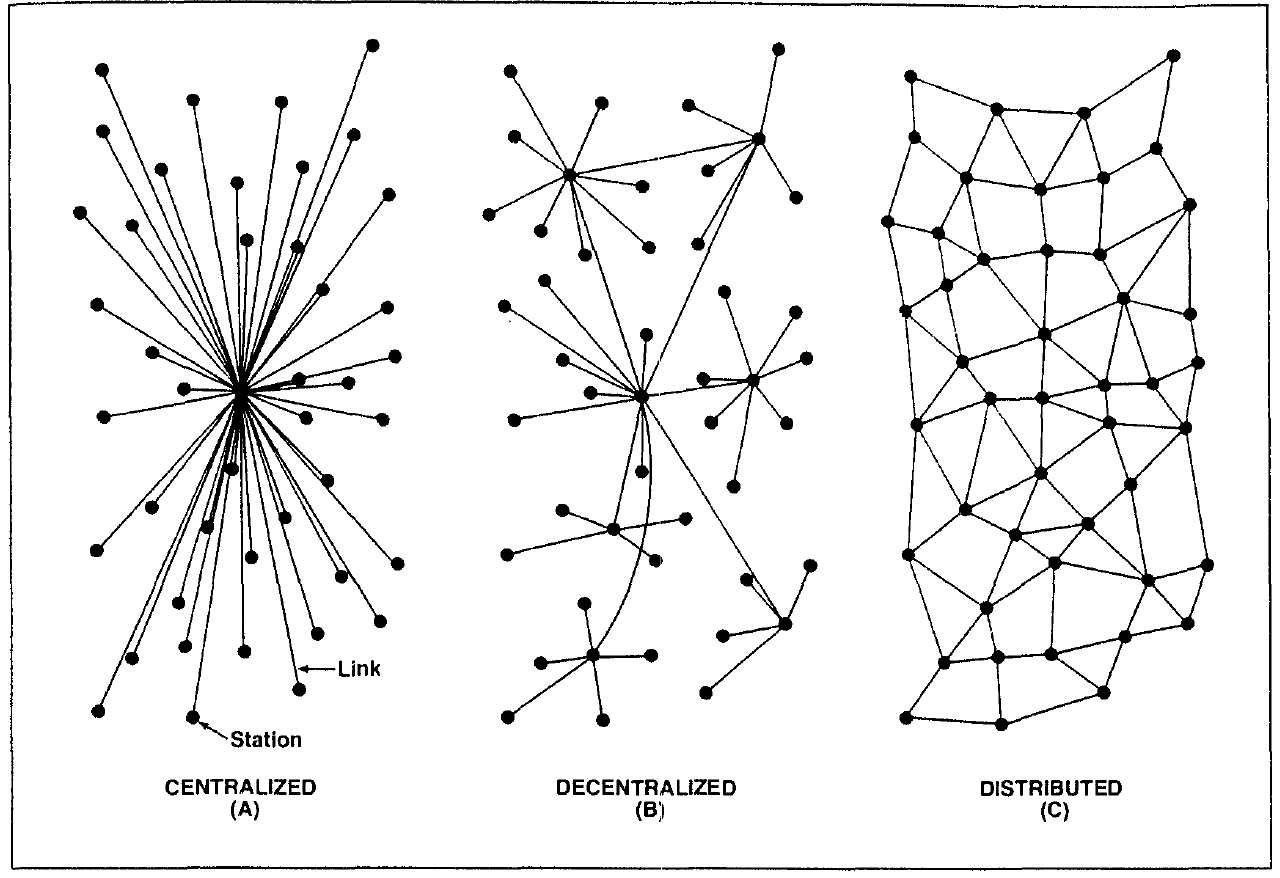
\includegraphics[width=0.8\textwidth]{networks}
  \end{center}
\end{frame}

\begin{frame}
  \frametitle{Peer-to-Peer Networks 2/2}
  \begin{itemize}
  \item In \textbf{centralized} systems, a successful attack on the \textbf{server}
    disables the whole system.
  \item In \textbf{decentralized} systems, a successful attack on a \textbf{hub}
    results in a temporary network partition, but the system remains
    operational.
  \item In \textbf{peer-to-peer} systems, a successful attack on a \textbf{peer}
    has no effect on the network \textit{if the network is big enough}.
  \item Examples: \textbf{Napster} and \textbf{BitTorrent}.
  \end{itemize}
\end{frame}

\begin{frame}
  \frametitle{Bitcoin Network 1/2}
  \begin{itemize}
  \item \textbf{Bitcoin Network} is a \textbf{peer-to-peer} network that
    consists on \textbf{Bitcoin nodes} that propagate blocks and transactions
    via the \textbf{gossip protocol} and validate them according to
    \textbf{consensus rules}.
  \item According to \href{https://bitnodes.io}{bitnodes.io}, Bitcoin network
    has approximately \textbf{21,000} \textit{reachable} nodes, compared to
    16,000 in 2022 and 10,000 in 2021.
  \item According to \href{https://luke.dashjr.org}{luke.dashjr.org}, estimated
    total number of \textbf{full} nodes (i.e. nodes that perform validation of
    chain data) is around \textbf{100,000} nodes.
  \end{itemize}
\end{frame}

\begin{frame}
  \frametitle{Bitcoin Network 2/2}
  \begin{itemize}
  \item According to \href{https://luke.dashjr.org}{luke.dashjr.org}, 71.62\% of
    all nodes run the most recent software (Bitcoin Core 28.x, 27.x).
  \end{itemize}
  \begin{center}
    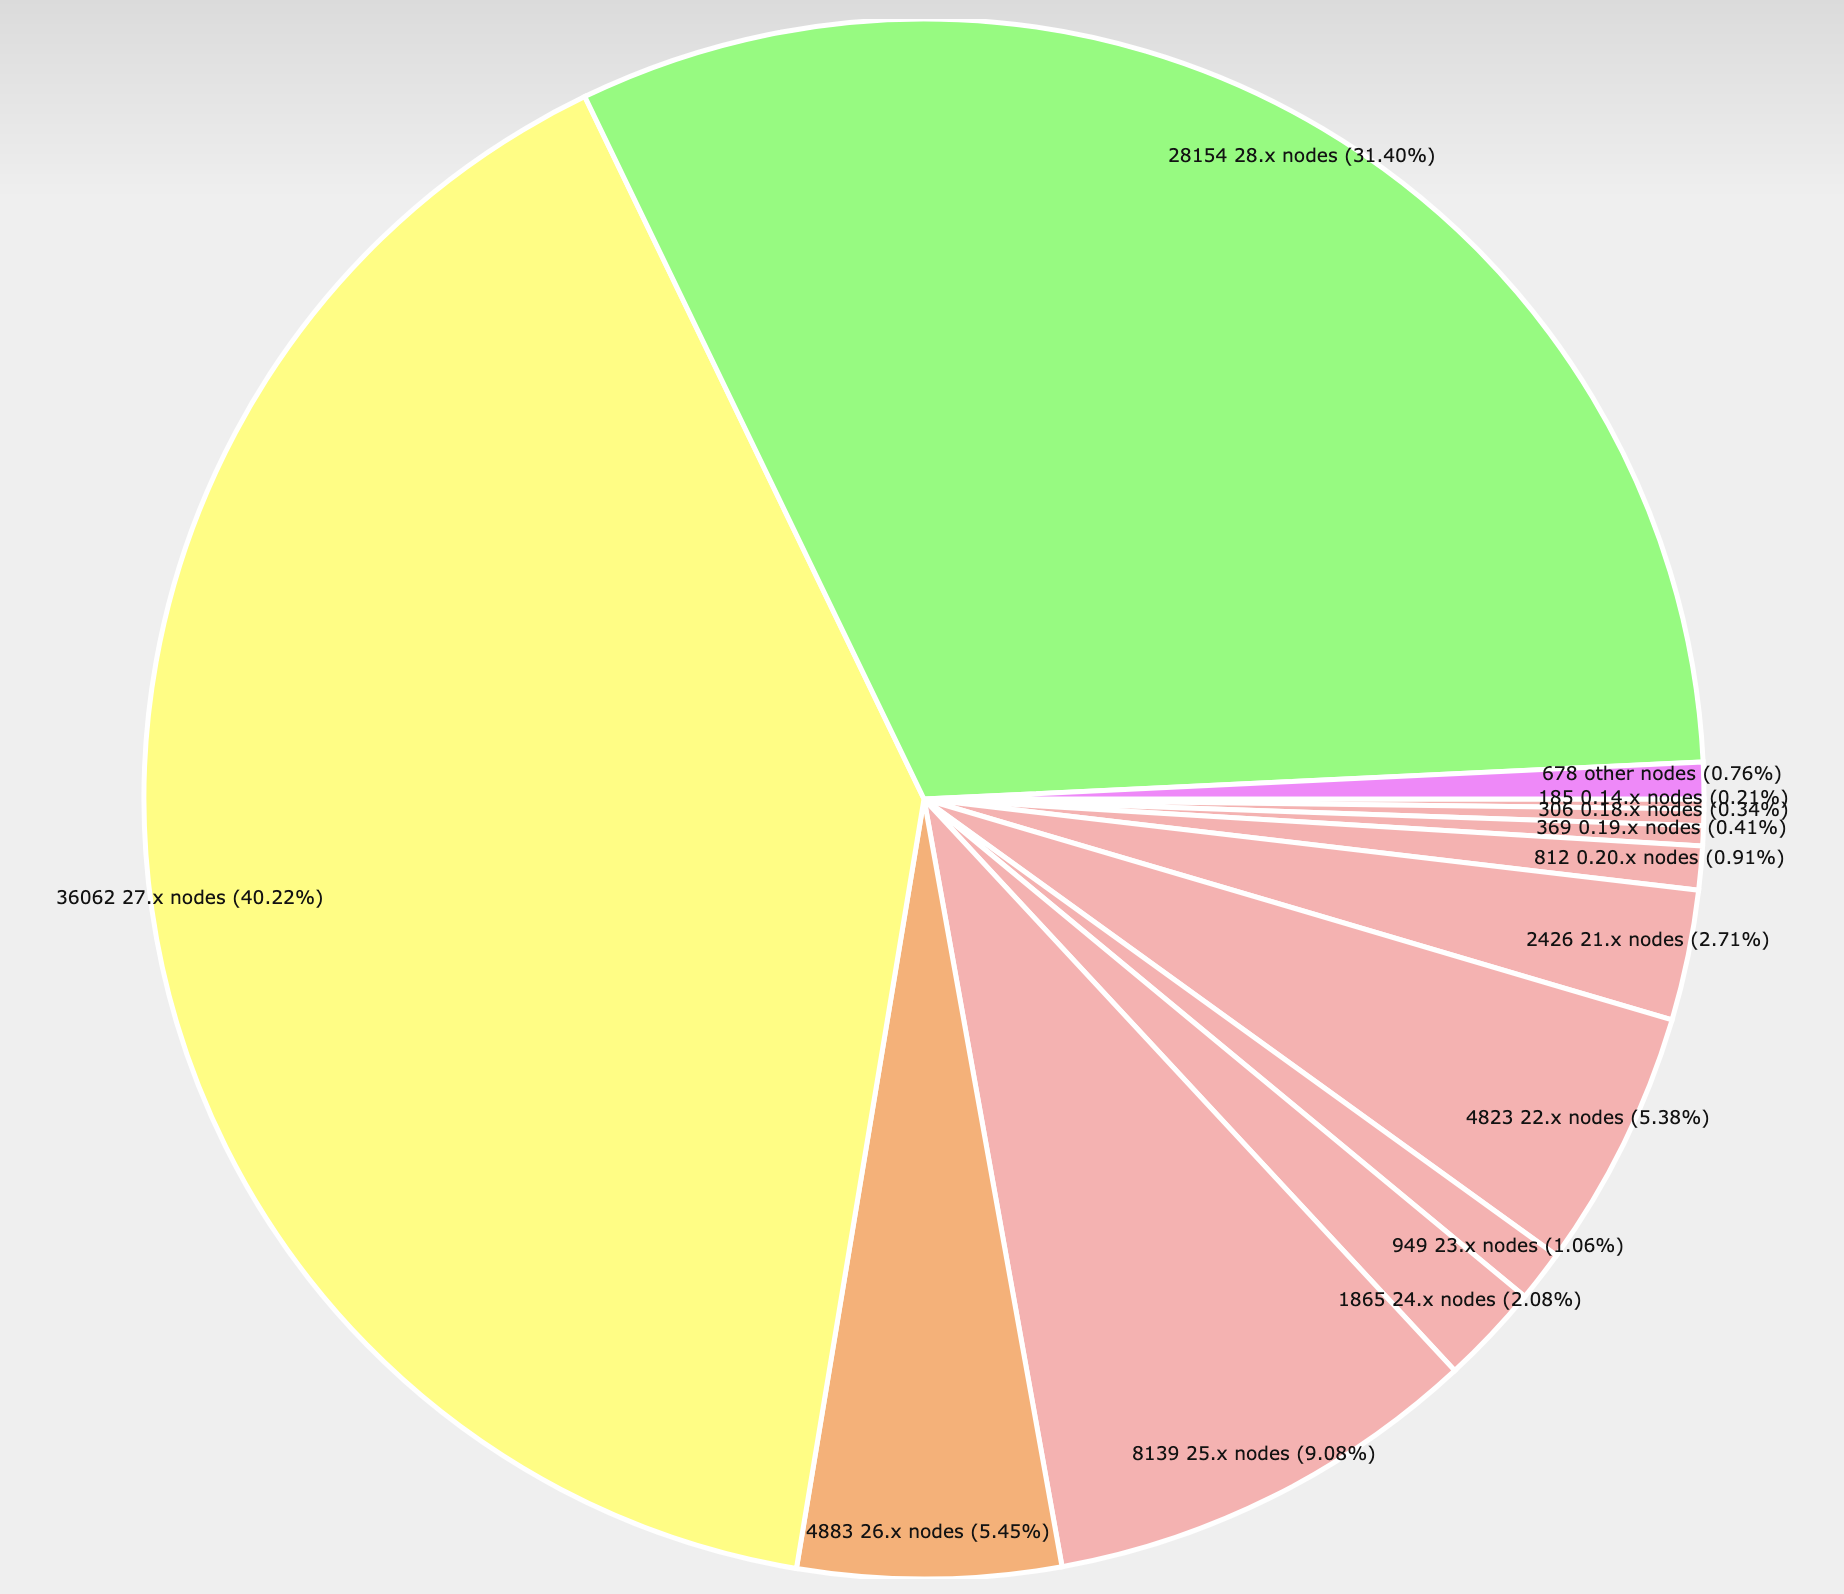
\includegraphics[width=0.7\textwidth]{nodes}
  \end{center}
\end{frame}

\begin{frame}
  \frametitle{Gossip Protocol}
  \begin{itemize}
  \item \textbf{Gossip protocol} (a.k.a. \textbf{epidemic protocol}) is a
    process of peer-to-peer communication that is based on the way
    \textit{epidemics} spread.
  \item \textbf{Receive information from one of their neighbours and pass it on
      to as much of their neighbours as possible.}
  \item \textbf{Bitcoin gossip protocol} is a gossip protocol for propagating
    new blocks and transactions as well as providing old blocks from storage to
    new peers on-demand.
  \end{itemize}
  \begin{center}
    \transduration<0-6>{0}
    \multiinclude[<+->][format=png, graphics={width=0.5\textwidth}]{gossip}
  \end{center}
\end{frame}

\begin{frame}
  \frametitle{Bitcoin Network Node}
  \begin{itemize}
  \item \textbf{Bitcoin node} is a member of Bitcoin network, a piece of
    software that executes the gossip protocol and validates blocks and
    transactions.
  \item A newly started Bitcoin node:
    \begin{itemize}
    \item initializes the connections to several nodes via DNS seeds,
    \item performs \textbf{initial block download} (\textbf{IBD}),
    \item builds necessary indices (UTXO set),
    \item starts listening for new blocks and transactions,
    \item rejects invalid blocks and transactions,
    \item accepts and re-broadcasts valid blocks and transactions.
    \end{itemize}
  \end{itemize}
\end{frame}

\begin{frame}
  \frametitle{Chain Reorganization 1/2}
  \begin{itemize}
  \item When a new block is received that does not belong to the current chain,
    node attempts to reconnect it to the chain by finding the \textbf{fork
      point}.
  \item Once the block is reconnected, \textbf{the chain that took more energy
      to build} (has the most cumulative \textbf{chainwork}) is chosen as the
    valid chain.
  \end{itemize}
  \begin{center}
    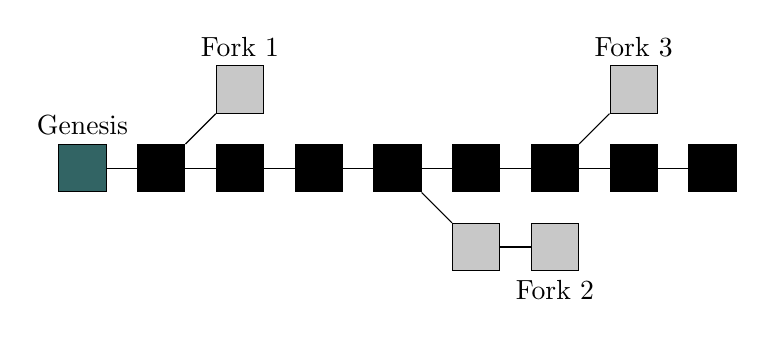
\begin{tikzpicture}
      % Define block size
      \def\blocksize{0.6}
      
      % Define colors
      \definecolor{mainchain}{RGB}{0,0,0}
      \definecolor{forkchain}{RGB}{200, 200, 200}
      \definecolor{genesis}{RGB}{50,100,100}

      % Genesis block
      \node[draw, fill=genesis, minimum size=\blocksize cm] (G) at (-1,0) {};

      % Main chain blocks
      \node[draw, fill=mainchain, minimum size=\blocksize cm] (B1) at (0,0) {};
      \node[draw, fill=mainchain, minimum size=\blocksize cm] (B2) at (1,0) {};
      \node[draw, fill=mainchain, minimum size=\blocksize cm] (B3) at (2,0) {};
      \node[draw, fill=mainchain, minimum size=\blocksize cm] (B4) at (3,0) {};
      \node[draw, fill=mainchain, minimum size=\blocksize cm] (B5) at (4,0) {};
      \node[draw, fill=mainchain, minimum size=\blocksize cm] (B6) at (5,0) {};
      \node[draw, fill=mainchain, minimum size=\blocksize cm] (B7) at (6,0) {};
      \node[draw, fill=mainchain, minimum size=\blocksize cm] (B8) at (7,0) {};

      % Forks
      \node[draw, fill=forkchain, minimum size=\blocksize cm] (F1) at (1, 1) {};
      \node[draw, fill=forkchain, minimum size=\blocksize cm] (F2) at (4,-1) {};
      \node[draw, fill=forkchain, minimum size=\blocksize cm] (F3) at (5,-1) {};
      \node[draw, fill=forkchain, minimum size=\blocksize cm] (F4) at (6, 1) {};

      % Connecting lines
      \draw[-] (G) -- (B1);
      \draw[-] (B1) -- (B2);
      \draw[-] (B2) -- (B3);
      \draw[-] (B3) -- (B4);
      \draw[-] (B4) -- (B5);
      \draw[-] (B5) -- (B6);
      \draw[-] (B6) -- (B7);
      \draw[-] (B7) -- (B8);

      % Fork connections
      \draw[-] (B1) -- (F1);
      \draw[-] (B4) -- (F2);
      \draw[-] (F2) -- (F3);
      \draw[-] (B6) -- (F4);

      % Labels
      \node[above] at (-1,0.3) {Genesis};
      \node[above] at (1, 1.3) {Fork 1};
      \node[below] at (5,-1.3) {Fork 2};
      \node[above] at (6, 1.3) {Fork 3};

    \end{tikzpicture}
  \end{center}
\end{frame}

\begin{frame}
  \frametitle{Chain Reorganization 2/2}
  \begin{itemize}
  \item \textbf{Chainwork} is the total number of hashes that are estimated to
    have been necessary to produce the current chain.
  \item \textbf{Headers-first IBD mode} makes IBD efficient by downloading the
    whole chain as headers first, and only then asking for whole blocks.
  \end{itemize}
\end{frame}

\begin{frame}
  \frametitle{Mempool}
  \begin{itemize}
  \item \textbf{Mempool} is an in-memory data structure that contains all known
    valid transactions that have not been included in any block yet.
  \item Nodes maintain a \textbf{combined UTXO set} that consists of all UTXOs
    in the chain and all UTXOs in the mempool.
  \item When a node receives a new valid transaction, it adds it to the mempool.
  \item When a node receives a new valid block, it removes all transactions in
    that block from the mempool.
  \item When a node receives a new transaction that conflicts with a transaction
    in its mempool, it rejects the new transaction unless it fits \textbf{RBF}
    (\textbf{Replace By Fee}) rules.
  \end{itemize}
\end{frame}

\begin{frame}
  \frametitle{Mining}
  \begin{itemize}
  \item \textbf{Miner nodes} are regular nodes that build new blocks from
    mempool transactions.
  \item A miner selects a number of transactions (2000-4000, usually sorted by
    fee) to build a \textbf{block template} within the \textbf{size limit}.
  \item Mining hardware performs a brute-force computation of the \textbf{Proof
      of Work} ($HASH256(Block) < Target$).
  \item When/if the block has been mined (i.e. PoW solution found), the miner
    broadcasts it to the network via the gossip protocol.
  \item If another miner ``finds'' a different block at the same time, the
    network eventually resolves the conflict via a chain reorganization.
  \end{itemize}
\end{frame}

\begin{frame}
  \frametitle{Transaction Lifecycle 1/2}
  \begin{itemize}
  \item A transaction \textbf{destroys} a subset of chain/mempool UTXOs and
    \textbf{creates} a set of new mempool UTXOs.
  \item A \textbf{finalized} valid transaction is propagated via gossip protocol
    to all nodes on the network.
  \item A transaction usually remains in the mempool until its fee exceeds the
    threshold for the next block.
  \item While in the mempool, a transaction can be ``bumped'' higher in the
    using
    \begin{itemize}
    \item \textbf{Replace By Fee} (\textbf{RBF}) or
    \item \textbf{Child Pays For Parent} (\textbf{CPFP}).
    \end{itemize}
  \end{itemize}
\end{frame}

\begin{frame}
  \frametitle{Transaction Lifecycle 2/2}
  \begin{itemize}
  \item Eventually a transaction is included in one of the blocks.
  \item Once the block mined and propagated through the network, every node in
    the network
    \begin{itemize}
    \item removes the transaction from the mempool,
    \item applies the transaction to the UTXO set (removes destroyed UTXOs and
      adds created ones).
    \end{itemize}
  \item At this point the transaction becomes \textbf{confirmed}.
  \end{itemize}
\end{frame}

\begin{frame}
  \frametitle{The End}
  \begin{center}
    Thank you!
  \end{center}
\end{frame}

\end{document}

%%% Local Variables:
%%% mode: latex
%%% TeX-master: t
%%% End:
